\subsection{Main Results: Test-Set Comparison}

Table~\ref{tab:main-results} reports test-set accuracy, mean per-class accuracy, and top-5 accuracy for every model we trained, sorted by mean per-class accuracy.

\begin{table}[H]
\centering
\small
\begin{tabular}{lcccr}
\toprule
Method & Test Acc (\%) & MPC Acc (\%) & Top-5 (\%) & Trainable params \\
\midrule
\textbf{VPT-Deep}              & \textbf{91.64} & \textbf{92.83} & \textbf{97.93} & \textbf{170{,}598} \\
Frozen ResNet18                & 88.52 & 90.82 & 96.85 & 10{,}545{,}766 \\
Label Smoothing ($\alpha{=}0.1$) & 87.27 & 89.40 & 96.16 & 11{,}228{,}838 \\
Label Smoothing + Strong Aug   & 86.40 & 88.24 & 95.82 & 11{,}228{,}838 \\
ResNet50                       & 85.93 & 88.07 & 96.70 & 23{,}717{,}030 \\
VPT-Shallow                    & 84.13 & 85.70 & 95.43 & 86{,}118 \\
Baseline                       & 84.42 & 86.11 & 94.84 & 11{,}228{,}838 \\
Strong Augmentation            & 84.42 & 86.11 & 94.84 & 11{,}228{,}838 \\
Deformable                     & 81.33 & 83.46 & 94.31 & 11{,}415{,}534 \\
MixUp ($\alpha{=}0.2$)         & 80.52 & 83.50 & 92.34 & 11{,}228{,}838 \\
Hybrid (ours)                  & 78.73 & 81.34 & 93.01 & 11{,}353{,}290 \\
Dilated                        & 75.95 & 78.53 & 91.41 & 11{,}228{,}838 \\
Depthwise                      & 57.03 & 59.71 & 81.54 & 1{,}623{,}270 \\
\bottomrule
\end{tabular}
\caption{Test-set results for every model we trained, sorted by mean per-class accuracy. VPT-Deep wins by a margin of more than two MPC points while training only $\sim$0.2\% of its backbone parameters.}
\label{tab:main-results}
\end{table}

Figure~\ref{fig:param-efficiency} plots the same data on a log-parameter axis. The two VPT variants sit in the top-left corner: highest accuracy at the smallest trainable parameter count.

\begin{figure}[H]
\centering
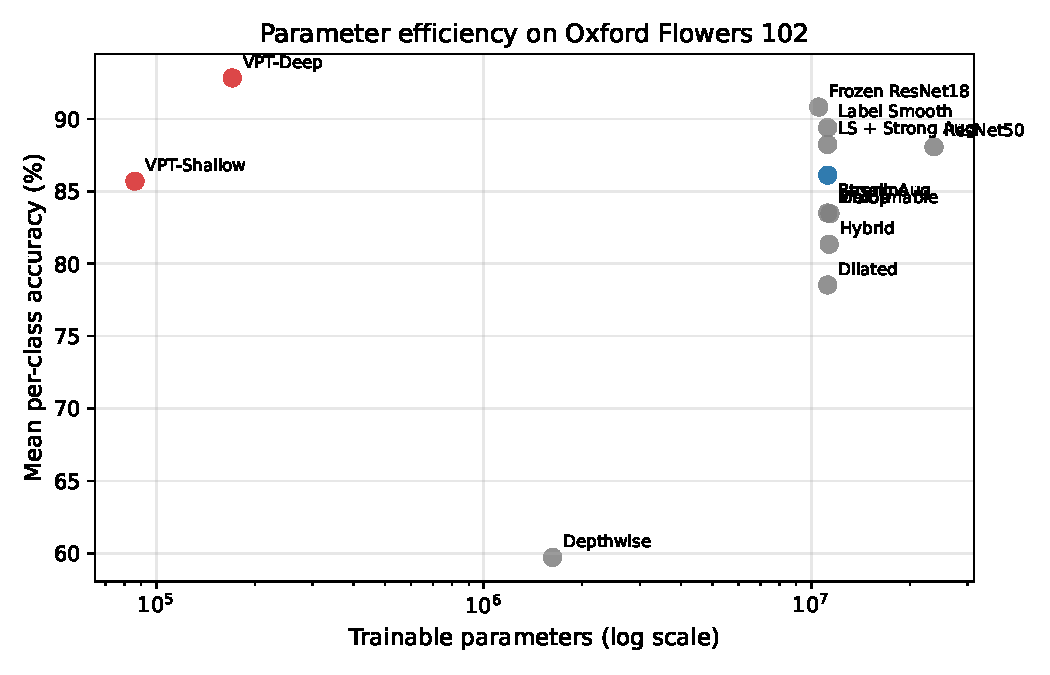
\includegraphics[width=0.8\textwidth]{figures/parameter-efficiency.pdf}
\caption{Mean per-class accuracy versus trainable parameter count. The VPT variants (red) achieve the best accuracy at the smallest parameter counts. CNN variants (grey) cluster in the middle-right region.}
\label{fig:param-efficiency}
\end{figure}

A few things stand out. VPT-Deep beats every CNN we tried, including the strongest regularized variant (Frozen ResNet18 at 90.82\% MPC). Among the CNNs, freezing early layers is the most useful single intervention; it outperforms both label smoothing and a $2\times$ larger ResNet50. None of our four architectural modifications to ResNet18 (dilated, deformable, hybrid, depthwise) reached the unmodified baseline. The most surprising failure was MixUp: a near-default regularizer in modern image pipelines, it dropped MPC accuracy by 2.6 points compared to the baseline.

\subsection{Few-Shot Learning Results}

Table~\ref{tab:fewshot} reports the best validation accuracy for each method as the per-class training budget shrinks from 10 to 1 image. Figure~\ref{fig:fewshot} plots the same numbers.

\begin{figure}[H]
\centering
\begin{minipage}{0.45\textwidth}
\centering
\small
\begin{tabular}{lcccc}
\toprule
Method & $k{=}1$ & $k{=}2$ & $k{=}5$ & $k{=}10$ \\
\midrule
\textbf{VPT-Deep}    & \textbf{46.4} & \textbf{68.8} & \textbf{84.9} & \textbf{93.6} \\
Frozen               & 35.1 & 65.8 & 81.5 & 91.7 \\
VPT-Shallow          & 37.8 & 57.2 & 77.5 & 86.1 \\
Baseline             & 35.2 & 59.3 & 79.6 & 88.3 \\
Deformable           & 27.0 & 54.2 & 77.5 & 84.6 \\
Hybrid               & 24.8 & 46.4 & 68.7 & 82.5 \\
Dilated              & 22.9 & 47.3 & 65.6 & 79.7 \\
Depthwise            & 7.0  & 12.8 & 39.4 & 60.8 \\
\bottomrule
\end{tabular}
\captionof{table}{Best validation accuracy (\%) at different training budgets.}
\label{tab:fewshot}
\end{minipage}\hfill
\begin{minipage}{0.53\textwidth}
\centering
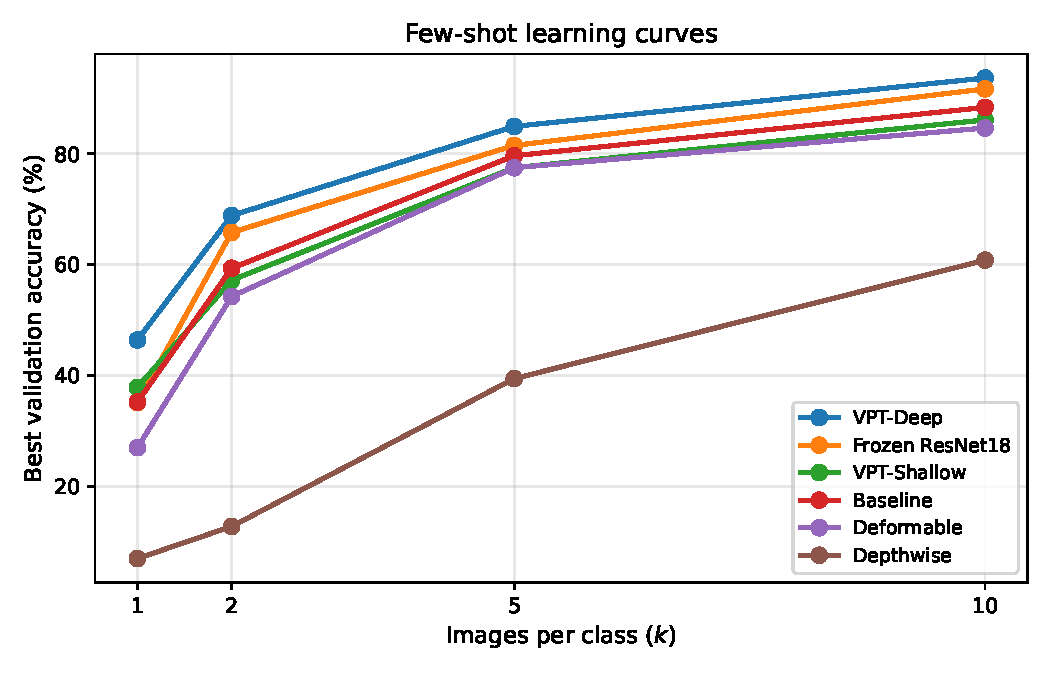
\includegraphics[width=\textwidth]{figures/fewshot-curves.pdf}
\captionof{figure}{Few-shot learning curves. VPT-Deep dominates at every $k$.}
\label{fig:fewshot}
\end{minipage}
\end{figure}

VPT-Deep wins at every $k$. The margin over the next best method (Frozen ResNet18) is roughly 1 point at $k=10$, 3 points at $k=5$, 3 points at $k=2$, and 11 points at $k=1$. The gap widens as data shrinks, which is the same pattern reported in the original VPT paper: with fewer labels, updating fewer parameters helps more. The baseline (full fine-tuning of 11M parameters) sits below both VPT and Frozen at small $k$ and only catches up at $k=10$. Depthwise collapses to near-random at $k=1$ (6.96\%) because it cannot reuse pre-trained weights and has nothing to learn from with one example per class.

\subsection{VPT Prompt Length Ablation and Triplet Loss}

Figure~\ref{fig:prompt-length} ablates the number of prompts per layer for VPT-Deep on the full training set. Accuracy increases monotonically from 91.08\% at $p = 1$ to 94.51\% at $p = 50$, with diminishing returns. The project handout also suggests triplet loss as an advanced loss function. We add a batch-hard triplet loss \citep{schroff2015facenet} on the L2-normalised CLS embeddings of VPT-Deep, with margin $0.5$ and weight $\alpha = 0.2$, giving combined loss $\mathcal{L} = \mathcal{L}_{\text{CE}} + \alpha \mathcal{L}_{\text{triplet}}$. Triplet loss raises validation accuracy by 0.4 points but does not change the test numbers (Table~\ref{tab:triplet}). We suspect the auxiliary objective tightens embeddings around the validation set without generalising further. Getting it to train at all required computing the triplet term in float32 outside the mixed-precision autocast; without that, we hit NaN losses within a few epochs.

\begin{figure}[H]
\centering
\begin{minipage}{0.5\textwidth}
\centering
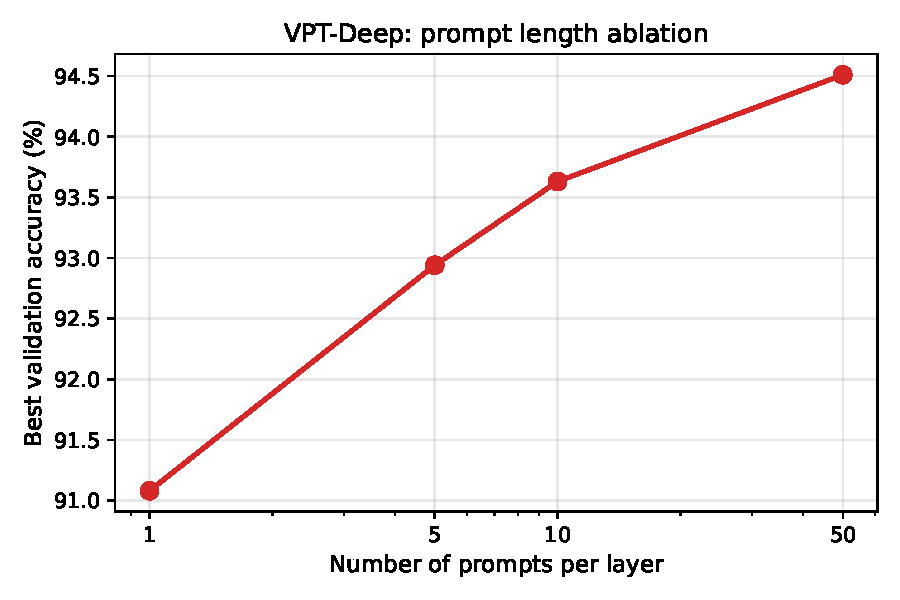
\includegraphics[width=\textwidth]{figures/prompt-length.pdf}
\captionof{figure}{VPT-Deep accuracy vs.\ prompt length.}
\label{fig:prompt-length}
\end{minipage}\hfill
\begin{minipage}{0.48\textwidth}
\centering
\small
\begin{tabular}{lccc}
\toprule
Method & Test & MPC & Val \\
\midrule
VPT-Deep             & 91.49 & 92.69 & 93.63 \\
\quad + Triplet ($\alpha{=}0.2$) & 91.49 & 92.69 & \textbf{94.02} \\
\bottomrule
\end{tabular}
\captionof{table}{Triplet loss helps validation but not test.}
\label{tab:triplet}
\end{minipage}
\end{figure}

\subsection{Regularization Ablation and Training Dynamics}

Table~\ref{tab:reg} isolates the effect of each regularization technique on the baseline ResNet18. Three of the four help, but only modestly; MixUp actively hurts. Combining label smoothing with strong augmentation gave less than label smoothing alone, so the two seem to compete for the same regularization slack. Figure~\ref{fig:training-curves} shows the validation accuracy curves: every model converges within 30--40 epochs under cosine annealing, VPT-Deep climbs fastest in the first 10 epochs (it has the stronger prior), and the CNNs hit 100\% training accuracy by epoch 20 while validation stays 5--14 points lower (the overfitting we expected). VPT-Deep uses $66\times$ fewer trainable parameters than the baseline yet ends up 6.7 MPC points higher.

\begin{figure}[H]
\centering
\begin{minipage}{0.45\textwidth}
\centering
\small
\begin{tabular}{lcc}
\toprule
Method & MPC (\%) & $\Delta$ \\
\midrule
Frozen \texttt{layer1+2}       & \textbf{90.82} & $+4.71$ \\
Label smoothing ($\alpha{=}0.1$) & 89.40 & $+3.29$ \\
LS + strong aug              & 88.24 & $+2.13$ \\
Baseline                     & 86.11 & --- \\
Strong aug only              & 86.11 & $+0.00$ \\
MixUp ($\alpha{=}0.2$)       & 83.50 & $-2.61$ \\
\bottomrule
\end{tabular}
\captionof{table}{Regularization effects on ResNet18.}
\label{tab:reg}
\end{minipage}\hfill
\begin{minipage}{0.53\textwidth}
\centering
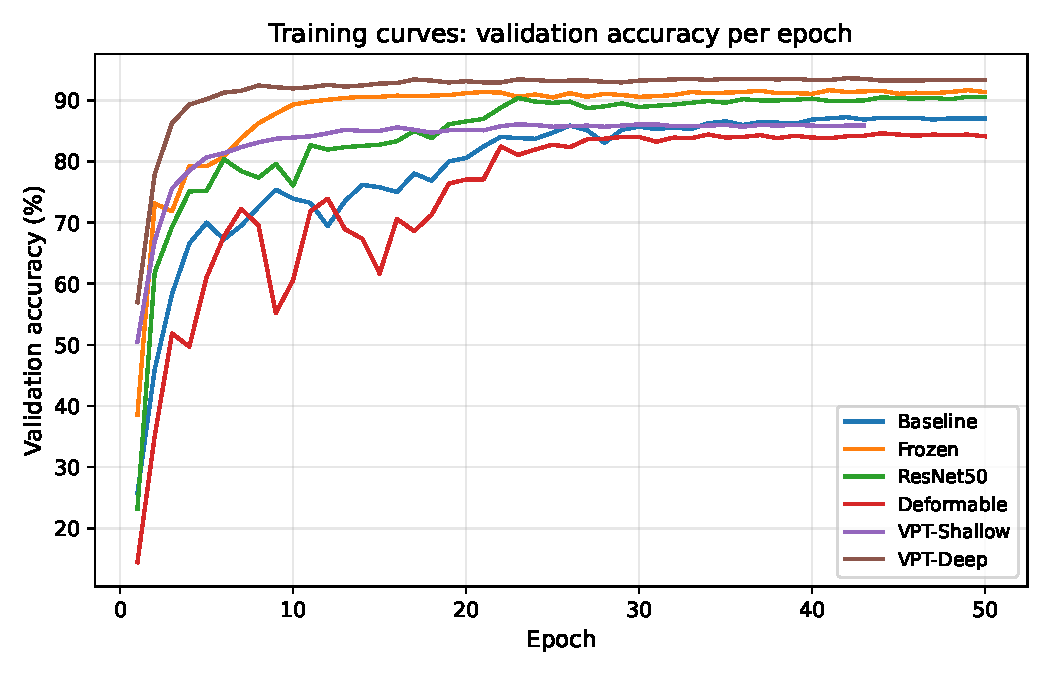
\includegraphics[width=\textwidth]{figures/training-curves.pdf}
\captionof{figure}{Validation accuracy per epoch.}
\label{fig:training-curves}
\end{minipage}
\end{figure}

\subsection{Test-Time Augmentation and Variance Across Seeds}\label{sec:seed-sweep}

For test-time augmentation we average the softmax predictions over five views (original, horizontal flip, $\pm 5^\circ$ rotation, $+10^\circ$ rotation). TTA improves every method by 0.4 to 0.9 points at no extra training cost (Table~\ref{tab:tta}). VPT-Deep with TTA reaches 93.27\% MPC, our highest test number. To address the single-seed limitation we re-train the three best methods with seeds 7 and 42 alongside seed 69 (Table~\ref{tab:seeds}). The relative ranking VPT-Deep $>$ Frozen $>$ Baseline holds at every seed, and standard deviations stay below one point.

\begin{figure}[H]
\centering
\begin{minipage}{0.62\textwidth}
\centering
\small
\begin{tabular}{lcccccc}
\toprule
& \multicolumn{2}{c}{Acc (\%)} & \multicolumn{2}{c}{MPC (\%)} & \multicolumn{2}{c}{Top-5 (\%)} \\
\cmidrule(lr){2-3} \cmidrule(lr){4-5} \cmidrule(lr){6-7}
Method & No & +TTA & No & +TTA & No & +TTA \\
\midrule
\textbf{VPT-Deep}   & 91.49 & \textbf{91.98} & 92.69 & \textbf{93.27} & 97.89 & \textbf{98.05} \\
Frozen              & 88.52 & 89.07 & 90.82 & 91.25 & 96.85 & 96.91 \\
Baseline            & 84.42 & 85.14 & 86.11 & 87.00 & 94.84 & 95.09 \\
\bottomrule
\end{tabular}
\captionof{table}{TTA effect on top three methods.}
\label{tab:tta}
\end{minipage}\hfill
\begin{minipage}{0.36\textwidth}
\centering
\small
\begin{tabular}{lc}
\toprule
Method & Mean $\pm$ std \\
\midrule
\textbf{VPT-Deep} & $93.07 \pm 0.49$ \\
Frozen            & $90.49 \pm 0.96$ \\
Baseline          & $87.97 \pm 0.28$ \\
\bottomrule
\end{tabular}
\captionof{table}{Best val acc across seeds 69, 7, 42.}
\label{tab:seeds}
\end{minipage}
\end{figure}

\noindent VPT-Deep also has the smallest spread across seeds (0.49 std), which fits with the idea that its tiny trainable parameter count limits how much any one initialisation can hurt or help.
